\documentclass[english,,man]{apa6}
\usepackage{lmodern}
\usepackage{amssymb,amsmath}
\usepackage{ifxetex,ifluatex}
\usepackage{fixltx2e} % provides \textsubscript
\ifnum 0\ifxetex 1\fi\ifluatex 1\fi=0 % if pdftex
  \usepackage[T1]{fontenc}
  \usepackage[utf8]{inputenc}
\else % if luatex or xelatex
  \ifxetex
    \usepackage{mathspec}
  \else
    \usepackage{fontspec}
  \fi
  \defaultfontfeatures{Ligatures=TeX,Scale=MatchLowercase}
\fi
% use upquote if available, for straight quotes in verbatim environments
\IfFileExists{upquote.sty}{\usepackage{upquote}}{}
% use microtype if available
\IfFileExists{microtype.sty}{%
\usepackage{microtype}
\UseMicrotypeSet[protrusion]{basicmath} % disable protrusion for tt fonts
}{}
\usepackage{hyperref}
\hypersetup{unicode=true,
            pdftitle={Principles for Describing or Explaining Process},
            pdfauthor={\ldots{}},
            pdfkeywords={\ldots{}.},
            pdfborder={0 0 0},
            breaklinks=true}
\urlstyle{same}  % don't use monospace font for urls
\ifnum 0\ifxetex 1\fi\ifluatex 1\fi=0 % if pdftex
  \usepackage[shorthands=off,main=english]{babel}
\else
  \usepackage{polyglossia}
  \setmainlanguage[]{english}
\fi
\usepackage{graphicx,grffile}
\makeatletter
\def\maxwidth{\ifdim\Gin@nat@width>\linewidth\linewidth\else\Gin@nat@width\fi}
\def\maxheight{\ifdim\Gin@nat@height>\textheight\textheight\else\Gin@nat@height\fi}
\makeatother
% Scale images if necessary, so that they will not overflow the page
% margins by default, and it is still possible to overwrite the defaults
% using explicit options in \includegraphics[width, height, ...]{}
\setkeys{Gin}{width=\maxwidth,height=\maxheight,keepaspectratio}
\IfFileExists{parskip.sty}{%
\usepackage{parskip}
}{% else
\setlength{\parindent}{0pt}
\setlength{\parskip}{6pt plus 2pt minus 1pt}
}
\setlength{\emergencystretch}{3em}  % prevent overfull lines
\providecommand{\tightlist}{%
  \setlength{\itemsep}{0pt}\setlength{\parskip}{0pt}}
\setcounter{secnumdepth}{0}
% Redefines (sub)paragraphs to behave more like sections
\ifx\paragraph\undefined\else
\let\oldparagraph\paragraph
\renewcommand{\paragraph}[1]{\oldparagraph{#1}\mbox{}}
\fi
\ifx\subparagraph\undefined\else
\let\oldsubparagraph\subparagraph
\renewcommand{\subparagraph}[1]{\oldsubparagraph{#1}\mbox{}}
\fi

%%% Use protect on footnotes to avoid problems with footnotes in titles
\let\rmarkdownfootnote\footnote%
\def\footnote{\protect\rmarkdownfootnote}


  \title{Principles for Describing or Explaining Process}
    \author{\ldots{}\textsuperscript{1}}
    \date{}
  
\shorttitle{PROCESS PRINCIPLES}
\affiliation{
\vspace{0.5cm}
\textsuperscript{1} ...}
\keywords{....\newline\indent Word count: 95}
\usepackage{csquotes}
\usepackage{upgreek}
\captionsetup{font=singlespacing,justification=justified}

\usepackage{longtable}
\usepackage{lscape}
\usepackage{multirow}
\usepackage{tabularx}
\usepackage[flushleft]{threeparttable}
\usepackage{threeparttablex}

\newenvironment{lltable}{\begin{landscape}\begin{center}\begin{ThreePartTable}}{\end{ThreePartTable}\end{center}\end{landscape}}

\makeatletter
\newcommand\LastLTentrywidth{1em}
\newlength\longtablewidth
\setlength{\longtablewidth}{1in}
\newcommand{\getlongtablewidth}{\begingroup \ifcsname LT@\roman{LT@tables}\endcsname \global\longtablewidth=0pt \renewcommand{\LT@entry}[2]{\global\advance\longtablewidth by ##2\relax\gdef\LastLTentrywidth{##2}}\@nameuse{LT@\roman{LT@tables}} \fi \endgroup}


\DeclareDelayedFloatFlavor{ThreePartTable}{table}
\DeclareDelayedFloatFlavor{lltable}{table}
\DeclareDelayedFloatFlavor*{longtable}{table}
\makeatletter
\renewcommand{\efloat@iwrite}[1]{\immediate\expandafter\protected@write\csname efloat@post#1\endcsname{}}
\makeatother
\usepackage{lineno}

\linenumbers

\authornote{\ldots{}.

Correspondence concerning this article should be addressed to \ldots{},
\ldots{}. E-mail: \ldots{}}

\abstract{
Begin here\ldots{}


}

\usepackage{amsthm}
\newtheorem{theorem}{Theorem}[section]
\newtheorem{lemma}{Lemma}[section]
\theoremstyle{definition}
\newtheorem{definition}{Definition}[section]
\newtheorem{corollary}{Corollary}[section]
\newtheorem{proposition}{Proposition}[section]
\theoremstyle{definition}
\newtheorem{example}{Example}[section]
\theoremstyle{definition}
\newtheorem{exercise}{Exercise}[section]
\theoremstyle{remark}
\newtheorem*{remark}{Remark}
\newtheorem*{solution}{Solution}
\begin{document}
\maketitle

We -- organizational psychologists -- are increasingly interested in
process and dynamic phenomena. Longitudinal studies are becoming more
prevalent in our literature and the number of time points they employ
appears to be growing. The empirical literature uses the term
\enquote{dynamics} at exponentially larger rates in recent years
(DeShon, 2012). A majority of published methods literature now focuses
on longitudinal data analysis (Aguinis, Pierce, Bosco, \& Muslin, 2009),
and there are many great reviews on the conceptual and methodological
issues related to dynamic and within-person models (Beal, 2015; Shipp \&
Cole, 2015; Wang, Zhou, \& Zhang, 2016). Moreover, this interest covers
many content areas, including self-regulation, leadership, and team
performance (Hardy, Day, \& Steele, 2018; Schaubroeck, Lam, \& Peng,
2016).

Given our interest in \enquote{process} phenomena, what distinguishes a
process from a non-process study? What are some fundamentals for people
wanting to study process? Consider the following studies and, while
reading, ask yourself which you feel appropriately represents process.
Imagine that we are interested in weight gain among US males who are 50
years or older, and to investigate it we conduct three longitudinal
studies. \textbf{Option A}. In the first, we find and report that the
average male gains one pound every year for the rest of his life. In the
second, we find and report a positive relationship between male weight
and caloric intake across time, and suggest that caloric intake has an
effect on weight. In the third, we propose that weight on any day is
determined by its value from the day before and the difference between
today's caloric intake and expenditure.

\textbf{Option B}. In the first, we model weight over time, find a
significant, positive trend, and suggest that the average male gains one
pound every year for the rest of his life. In the second, we model
weight and the number of consumed calories over time, find a
significant, positive relationship between them, and suggest an effect
of caloric intake and weight. In the third, we model initial weight,
weight, and the number of consumed and expended calories over time and
suggest that weight is a function of prior weight and difference between
caloric intake and expenditure.

Which of these is a process study? Where is the line between explaining
a process versus describing its manifest properties? What are the
different ways that we can represent it? In this paper we call attention
to these questions and provide a number of principles to help
researchers convey some components of process. We are agnostic as to
which of the studies above is a \enquote{true} process study -- we feel
that, at the current state of our literature, it is more important to
raise attention to the issue and initiate discussion and debate over the
coming years. All three studies have meaningful pieces to convey, what
we want to do here is give researchers the tools to talk about each
aspect. We do so in two parts.

In the first section we contrast process with other, \enquote{over time}
concepts. There are loose and formal ways to use terms and notions about
behavior over time, and we point out the differences to locate process
within that concept map. We then provide a definition drawn from
Pettigrew (1992) and Pettigrew (1997) that orients the rest of the
paper.

In the second section we discuss principles for either describing or
explaining processes. The principles come from a number of areas,
including mathematics, systems theory, dynamics, and computational
modeling, and they are all ways to represent and describe relationships
over time at different levels of abstraction. For example, we could use
a difference equation to explain the trajectory of one variable, or we
could use terms like trend or cycles that describe its manifest behavior
but through a different lens. We want to point researchers to principles
that they can use to represent or convey variables/behavior over time --
regardless of whether they are truly causal or non causal explanations.

(\textbf{Not clean paragraph} - may not even need it). We provide
several contributions in doing so. First, we believe our discussion will
help researchers augment their current approach to explaining process.
It can be helpful to be exposed to different approaches, provide ideas
etc., and we hope our paper provides new ideas to seasoned researchers
in this area. Second, although there is a substantial amount of
literature on mathematical process principles and dynamics, it is
sophisticated and technical. Much of this work is not easily accessible
to researchers with the usual methodological and statistical background
obtained from doctoral level training in OP/OB; we want to help distill
it. Finally, we discuss ways to study process for researchers who may
not want to want to develop sophisticated math or computational models.
Some people claim that math is the only option. For example, Pearl
(2009) states that any explanation \enquote{worthy of the title theory
must be able to represent causal questions in some mathematical
language} (p.~102). There is also some pressure to produce computational
theories. For example, VANCOUVER COMP MODELS ARE BETTER; AND KOZLOWSKI
COMP FRAMEWORKS ARE BETTER. But there are not many comp modelers in
organizational psychology (vancouver orm); and the social sciences do
not emphasize mathematics as much as some of the more physical sciences
(vancouver orm). Moreoever, Renee Thom points out that sometimes
qualitative representations produce more error than their quantitative
counterparts but nonetheless are better clues to the underlying process.
We do not claim that one approach is better or worse than another; we
simply want to describe process principles from different domains to
give researchers alternative ways of talking about, specifying, and
representing process behavior.

\hypertarget{process}{%
\section{Process}\label{process}}

Before jumping to a definition of process it is helpful to consider
other, related concepts.

\hypertarget{dynamics}{%
\subsubsection{Dynamics}\label{dynamics}}

Dynamics refers to a specific branch of mathematics/mechanics, but the
term is used in different ways throughout our literature. It is used
informally to mean \enquote{change}, \enquote{fluctuating,}
\enquote{volatile,} \enquote{longitudinal,} or \enquote{over time}
(among others), whereas formal definitions in our literature are
presented within certain contexts. Wang (2016) defines a dynamic
\emph{model} as a \enquote{representation of a system that evolves over
time. In particular it describes how the system evolves from a given
state at time \emph{t} to another state at time \(t + 1\) as governed by
the transition rules and potential external inputs} (p.~242). Vancouver,
Wang, and Li (2018) state that dynamic \emph{variables} \enquote{behave
as if they have memory; that is, their value at any one time depends
somewhat on their previous value} (p.~604). Finally, Monge (1990)
suggests that in dynamic \emph{analyses}, \enquote{it is essential to
know how variables depend upon their own past history} (p.~409).

The crucial notion to take from dynamics, then, is memory. When the past
matters, and future states are constrained by where they were at prior
points in time, dynamics are at play.

\hypertarget{longitudinal}{%
\subsubsection{Longitudinal}\label{longitudinal}}

Longitudinal is a broad term that is usually paired with one additional
term to refer to an investigation's method, data, or aim. A study that
uses a longitudinal \emph{method} is different from a cross-sectional
design due to the number of observations, such that longitudinal designs
employ repeated observations, whereas cross-sectional studies do not.
Longitudinal \emph{data} are repeated observations on multiple units,
whereas panel or time series data -- the common data structure in
economics -- are repeated observations on one unit.

The other distinction surrounding longitudinal studies is what
researchers hope to discover by using them. Ployhart and Vandenberg
(2010) state that \enquote{longitudinal research emphasizes the study of
change and contains at minimum three repeated observations on at least
one of the substantive constructs of interest} (p.~97). Similarly,
Baltes and Nesselroade (1979) note, \enquote{the study of phenomena in
their time-related constancy and change is the aim of a longitudinal
methodology} (p.~6). Both of these definitions reveal the recent
tendency to focus on change in longitudinal studies. For example, a
longitudinal investigation could observe increasing or decreasing
trajectories (or other forms of change) across time. This change
emphasis is likely due to the increasing knowledge and application of
growth models, where change is the main interest.

\hypertarget{process-1}{%
\subsubsection{Process}\label{process-1}}

We presented the notions above to help pinpoint what process refers to.
Dynamic systems have memory, where current states are driven to future
states by transition rules and external inputs. Longitudinal studies
collect data on multiple units across time, and some suggest that they
ought to emphasize change. Process is about sequences of events with or
without memory and with or without change. Pettigrey (1997) provides a
formal definition: process is \enquote{a sequence of individual and
collective events, actions, and activities unfolding over time in
context} (p.~2).

This definition is consistent with sentiments found in Ilgen and Hulin
(2000). These authors indirectly define process by describing their
dissatisfaction with static research. They compare (some) OP/OB research
to individual snapshots of behavior that -- even if compiled and
aggregated to form a longitudinal study -- only reveal fleeting glances
of the flow of the system. \enquote{Frozen moments do not
capture\ldots{}a process, nor do statistical interactions make a
sequence} (71). Process, then, seems to entail sequences of events that,
as stated above, must be couched in context.

Another point we want to reiterate is how words like \enquote{dynamics,}
\enquote{change,} and \enquote{process} tend to be coupled. It is common
to pair two or more of these terms with a phrase like \enquote{the
dynamic process.} But each of these words has a precise meaning.
Dynamics is used for systems or variables with memory. Growth describes
the systematic increase or decrease of a variable or system over time.
Change has been used in two ways. It is sometimes used synonymously with
growth: systematic increase or decrease. At other times, researchers
partial prior observations of their dependent variable and in a
regression model to emphasize the effect of an IV on the change in the
DV (e.g., Johnson, Lanaj, \& Barnes, 2014). In this second way, change
does not mean \enquote{growth} but instead, \enquote{how a variable is
different from the last point in time.}

Process is distinct from each of these terms, and it does not need to be
paired with any. Processes can grow, or they can not grow; they can
change or not change; they can contain dynamics or no dynamics. Stated
differently, \enquote{no change} in not synonymous with \enquote{not
process.} We can still find process in behavior that does not change
over time.

Having discussed the differences between terms like process,
longitudinal, and dynamics, we now unpack the principles. All of these
are ways to represent process behavior -- to talk about how things
unfold over time. Some are explanatory, whereas others simply describe
manifest behavior while remaining agnostic to the undiscovered true
underlying mechanism, but all help convey process behavior.

\hypertarget{systems-theory-principles}{%
\section{Systems Theory Principles}\label{systems-theory-principles}}

We start with principles from systems theory -- a gentle place to begin
given that some of the terms will overlap with the growth modeling
literature.

\hypertarget{stocks-and-flows}{%
\subsection{Stocks and Flows}\label{stocks-and-flows}}

One common approach to explaining how things happen over time is to
identify stocks and flows. Meadows (2008) defines both with the
following:

\begin{quote}
A stock is a store, a quantity, an accumulation of material or
information that has built up over time. It may be the water in a
bathtub, a population, the books in a bookstore, the wood in a tree, the
money in a bank, your own self confidence. A stock does not have to be
physical. Your reserve of good will toward others or your supply of hope
that the world can be better are both stocks.
\end{quote}

\begin{quote}
Stocks change over time through the actions of flows. Flows are filling
and draining, births and deaths, purchases and sales, growth and decay,
deposits and withdrawals, successes and failures. A stock, then, is the
present memory of the history of changing flows within the system (18).
\end{quote}

\noindent That last sentence is what makes a stock imply behavior over
time. We speak about stocks by both referring to what they contain right
now but also how they have developed and where they are likely to go.
Also note that stocks do not have to change.

The behavior of a stock -- whether it rises, falls, or remains the same
-- depends on the nature of flows. We can learn about stock behavior by
subtracting outflows from inflows. Doing so leads to three general
principles about stocks. They will (Cronin, Gonzalez, \& Sterman, 2009):
(1) rise when inflows exceed outflows, (2) fall when outflows exceed
inflows, and (3) remain the same when inflows equal outflows. In other
words, stocks change with respect to the summative properties of their
flows. Stocks also set the pace for the cumulative rhythm of the system.
Even when flows are changing rapidly, the stock may change slowly
because accumulation occurred over a long period of time.

Figure \ref{stocks} plots a simple stock and flow system over 20 time
periods.

\begin{center}

---------------

Insert Figure \ref{stocks} Here

---------------

\end{center}

\begin{figure}
\centering
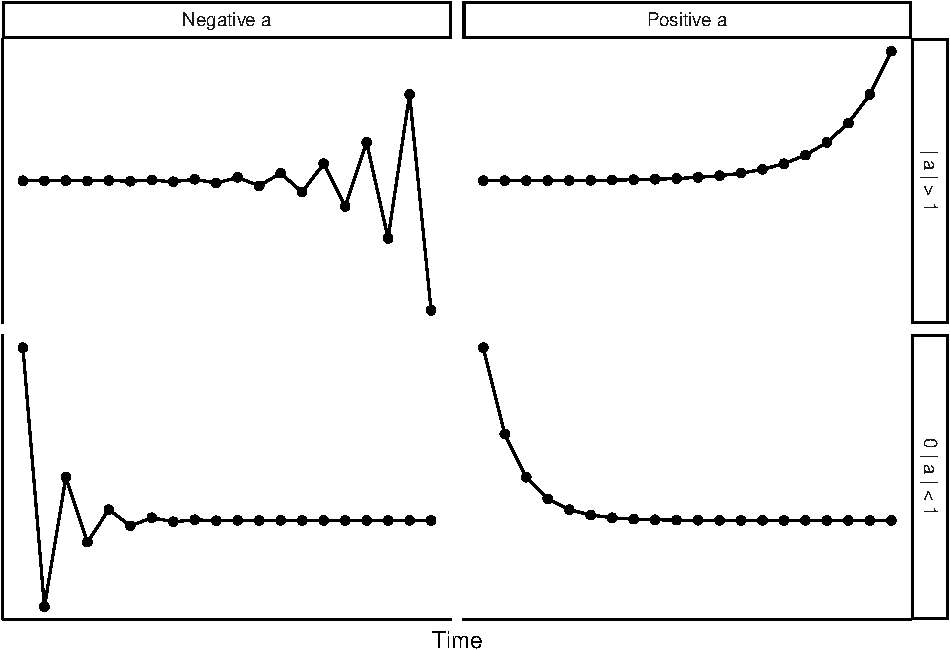
\includegraphics{figs/unnamed-chunk-6-1.pdf}
\caption{\label{fig:unnamed-chunk-6}the ol stock system\label{stocks}}
\end{figure}

\noindent Beginning at the first time point, inflows are equal to
outflows and the stock therefore sits at zero. Over the first ten time
points, however, outflows remain the same whereas inflows increase. With
inflows exceeding outflows the stock also increases up until time point
ten. At this time, inflows drop back down to five whereas outflows
increase -- leading to a large reduction in the stock. As outflows
continue to rise over time -- with no counterbalancing movement from the
inflow -- the stock ultimately decreases.

Systems theory uses stocks and flows as general labels for each of the
things in the system. Above, we described the behavior of the stocks and
flows with simple terms -- increasing, decreasing, or constant. Systems
theory also provides a more systematic way of describing trajectories
and explaining behavior over time. These are unpacked in an excellent
paper by Monge (1990), and the framework includes trend, magnitude, rate
of change, and periodicity. These are shown respectively in figure
\ref{monge}.

\begin{figure}
\centering
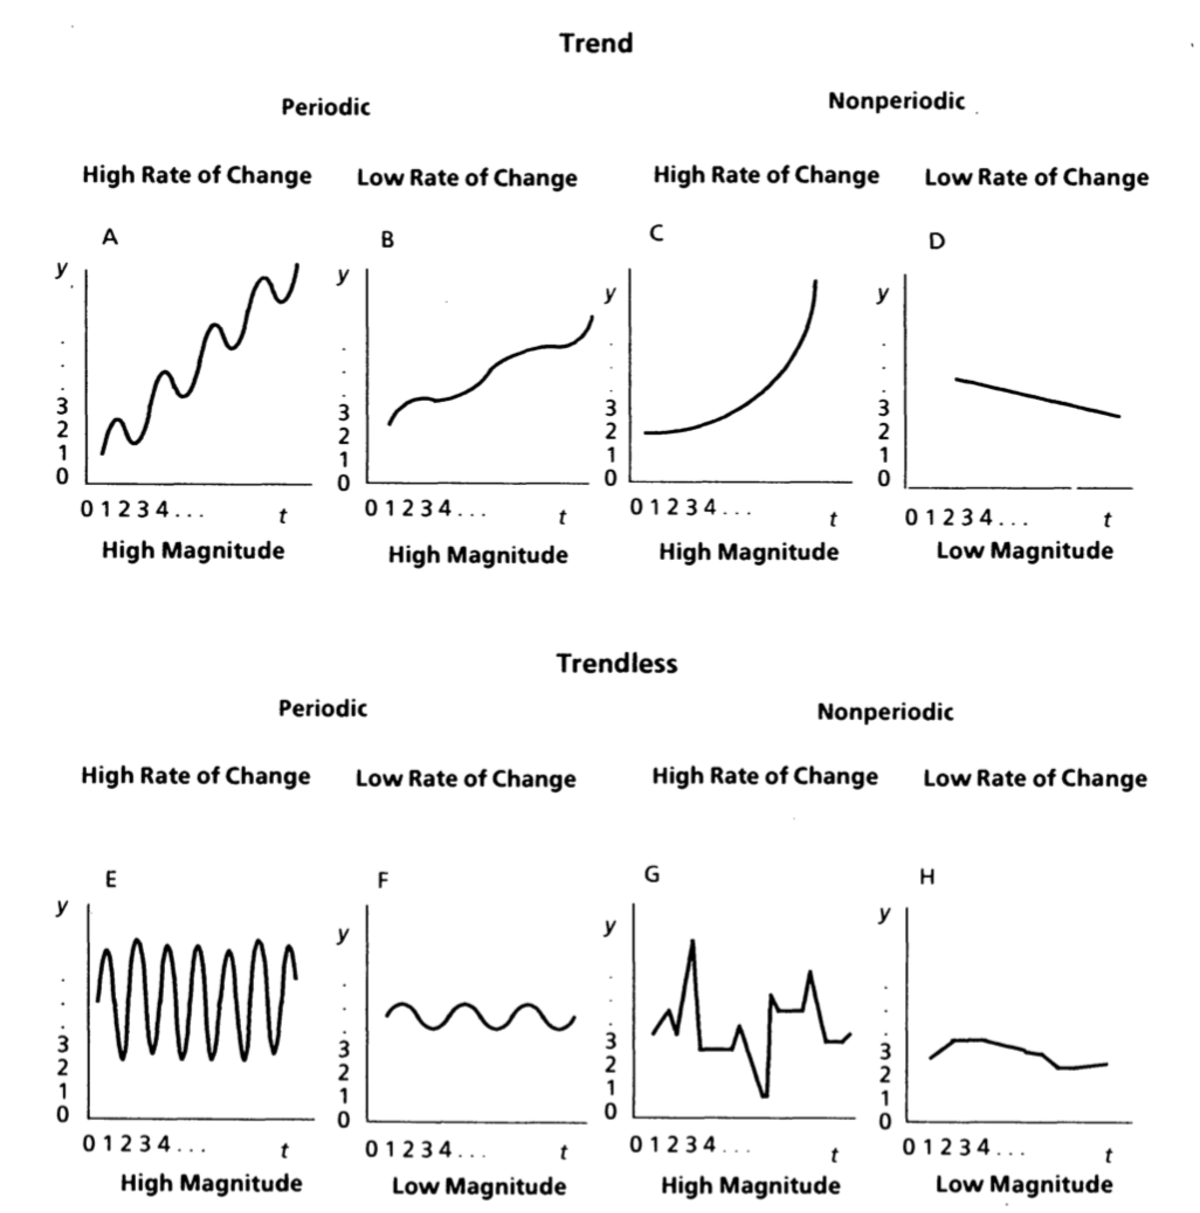
\includegraphics{figs/unnamed-chunk-7-1.pdf}
\caption{\label{fig:unnamed-chunk-7}monge image\label{monge}}
\end{figure}

\begin{center}

---------------

Insert Figure \ref{monge} Here

---------------

\end{center}

\hypertarget{trend}{%
\subsection{Trend}\label{trend}}

Dividing figure \ref{monge} into two portions -- the top and bottom --
reveals differences in trend. All of the panels on the top of the figure
have trend, whereas those on the bottom do not. Trend is the systematic
increase or decrease of a variable over time.

\hypertarget{magnitude}{%
\subsection{Magnitude}\label{magnitude}}

Magnitude is the level, value, or amount of the variable at each time
point -- the number on the \(y\) axis at each respective point in time.
For example, in panel \emph{C} of figure two the magnitude is low at
times 1, 2, and 3, but is high at later points in time. Additionally,
panel \emph{E} and \emph{F} have the same magnitude if we average their
values over time, but panel \emph{E} contains both high and low
magnitude, whereas the magnitude for the trajectory in panel \emph{F}
remains relatively constant.

\hypertarget{rate-of-change}{%
\subsection{Rate of Change}\label{rate-of-change}}

Monge (1990) refers to rate of change as \enquote{How fast the magnitude
increases or decreases per one unit of time.} Panels \emph{G} and
\emph{H} reveal differences in rates of change.

\hypertarget{periodicity}{%
\subsection{Periodicity}\label{periodicity}}

Periodicity is the amount of time before a pattern repeats itself, and
it is equivalent to the term cycle. The most important piece about
periodicity is that it must be couched with \enquote{controlling for
trend.} Notice that panel \emph{A} is periodic because, after
controlling for trend, there are repeated patterns over time.

\hypertarget{two-variables}{%
\subsection{Two Variables}\label{two-variables}}

It is of course possible to combine these notions when researchers are
studying processes with more than one variable. For example, a
researcher might describe the magnitude in their presumed dependent
variable with respect to the magnitude of their independent variable, or
the rates of change across the system of variables. When we turn to the
behavior and relationships among two or more variables -- i.e., a system
of variables -- a few additional principles are available.

\hypertarget{lags}{%
\subsection{Lags}\label{lags}}

How long does it take for the presumed independent variable to produce
an effect on the outcome? This is the notion of lag.

\hypertarget{permanence}{%
\subsection{Permanence}\label{permanence}}

Once the effect happens, how long does it last? That is, if the
independent variable causes the dependent variable to change to a new
value, does the dependent value remain at that new value indefinitely?

\hypertarget{feedback-loops}{%
\subsection{Feedback Loops}\label{feedback-loops}}

Systems theory researchers often convey process by using feedback loops.
Feedback loops describe processes where a variable eventually relates
back to itself.

There are two common ways to describe the behavior of a focal variable
within a feedback loop. When feedback causes the variable to move in the
opposite direction than it initially moved, this is known as negative
feedback, deviation counteraction, or a balancing feedback loop
(Meadows, 2008; Monge, 1990). Here, an initial increase in \(x\) leads
to subsequent changes in the system that, through time, eventually cause
\(x\) to decrease. Now that \(x\) has gone down, more changes happen in
the system that, through time, eventually cause \(x\) to increase.

When feedback, instead, causes the variable to move in the same
direction that it initially moved, this is known as postive feedback,
deviation ampliciation, or a reinforcing feedback loop (Meadows, 2008;
Monge, 1990). Here, changes in \(x\) in one direction lead to eventual
changes in \(x\) in the same direction and thus produce exponential,
explosive, or amplifying behavior. Of course, we can also identify
whether there is positive or negative feedback for every variable in the
system.

\hypertarget{examples}{%
\subsection{Examples}\label{examples}}

People from our literature using these terms and principles to explain
something. Study 1 measured X and Y and described trend. Study 2
measured X and Y and talked about cycles. Study 3 measured X and Y and
reported lags.

\hypertarget{summary}{%
\subsection{Summary}\label{summary}}

These systems theory notions are valuable tools to explain and describe
process. Note that we did not cover everything to keep the reading
concise and consistent. For example, ({\textbf{???}}) also covers
discontinuous systems, so please refer to his excellent paper for an
even deeper discussion. Now we turn to mathematics and dynamics and
describe principles from these domains that are used to explain or
describe process.

\hypertarget{mathematics-and-dynamics-principles}{%
\section{Mathematics and Dynamics
Principles}\label{mathematics-and-dynamics-principles}}

\hypertarget{difference-equations}{%
\subsection{Difference Equations}\label{difference-equations}}

In mathematics, a basic representation of a process over time is a
difference equation:

\begin{equation}
\label{basicD}
y_{t} = y_{t - 1}
\end{equation}

\noindent where \(y_{t}\) represents \(y\) now and \(y_{t-1}\) is the
variable at the prior time point. Here, the value of \(y\) is the same
at each \(t\), and the emergent behavior would be a flat line across
time. In systems theory terms, there would be no trend.

Although equation \ref{basicD} seems simple, it introduces a fundamental
concept in dynamics: memory. The variable now depends on where it was in
the past. It is constrained, there are boundaries on where it can go.

As we add terms to this basic difference equation the behavior of the
variable becomes more complex. Adding a forcing constant, \emph{c} in
equation \ref{basicD} produces positive or negative trend depending on
whether \emph{c} is, respectively, positive or negative. For example,
the following equation:

\begin{equation}
\begin{split}
\label{diffC}
y_{t} &= y_{t-1} + c \\ 
c &= -4
\end{split}
\end{equation}

\noindent produces a line that decreases by four units at each time
point.

The next level of complexity comes from autoregressive terms, which
represent the extent to which the variable relates to itself over time.
Here,

\begin{equation}
\begin{split}
\label{diffA}
y_{t} &= a y_{t-1} \\ 
a &= 0.5
\end{split}
\end{equation}

\noindent the variable is described over time but it does not retain the
same value at each \(t\). Instead, the variable is \emph{similar} over
time and the autoregressive term, \(a\), describes the extent of that
similarity. In equation \ref{diffA}, \(a\) is 0.5, meaning that the
relationship between the variable now and itself at the next time point
will be 0.5.

There are fundamental behaviors of dynamic variables based on their
autoregressive terms, and these are shown in figure \ref{dynamics_plot}.
The top row of figure \ref{dynamics_plot} shows the trajectory of
variables with autoregressive terms that are greater than one in
absolute value. These large terms produce explosive behavior --
exponential growth when \(a\) is positive and oscillating chaos when
\(a\) is negative. When the autoregressive term falls between zero and
one in absolute value, conversely, the variable converges to equilibrium
-- shown in the bottom two panels. Either the variable oscillates at a
decreasing rate until it reaches equilibrium (when \(a\) is negative) or
it converges there smoothly (when \(a\) is positive).

\begin{figure}
\centering
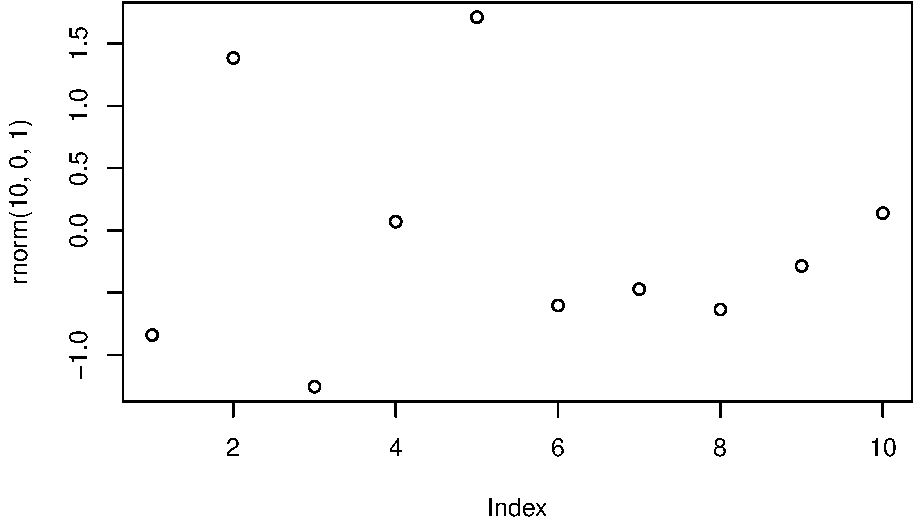
\includegraphics{figs/unnamed-chunk-8-1.pdf}
\caption{\label{fig:unnamed-chunk-8}dynamic equilibrium
fig\label{dynamics_plot}}
\end{figure}

\begin{center}

---------------

Insert Figure \ref{dynamics_plot} Here

---------------

\end{center}

\hypertarget{equilibrium}{%
\subsection{Equilibrium}\label{equilibrium}}

Notice that we introduced a new term in our description above:
equilibrium. Equilibrium describes the state of a variable that no
longer changes unless disturbed by an outside force. It can also be used
to describe multiple variable systems -- where equilibrium again means
that the state remains constant unless disturbed by an outside force,
but here state refers to the the entire system (i.e., all of the
variables). In \emph{static} equalibriums, the system has reached a
point of stability with no change, whereas \emph{dynamic} equilibrium
refers to systems with changes and fluctuations but no net change. That
is, the variables fluctuate across time in periodic ways but the general
state of the system does not diverge so as to change the behavior of the
entire system.

Predator-prey relationships are a typical example of a system in dynamic
equilibrium. For example, consider a predator-prey relationship between
bobcats and rabbits. As the rabbit population increases, the amount of
available food for the bobcats goes up. Over time, this raises the
population of the bobcats as well. Now with a greater bobcat population,
the rabbit population decreases because more are being killed. Over
time, this reduction in food opportunity decreases the bobcat
population. This back and forth oscillating pattern between variables
describes a dynamic equilibrium. The variables change and there may be
random disturbances to the system across time, but the net dynamics of
the system remain stable -- and therefore this situation is still called
\enquote{equilibrium.}

\hypertarget{stochastics}{%
\subsection{Stochastics}\label{stochastics}}

Our route so far has been deterministic -- the mathematical
representations do not contain error. When we want to convey a process
with error we can consider a host of additional principles. Stochastics,
stated simply, refers to processes with error. Consider our simple
difference equation from above, adding an error component produces:

\begin{equation}
\label{diffE}
y_{t} = a y_{t-1} + c + e_{t}
\end{equation}

\noindent where all terms are defined above but \(e_{t}\) represents an
error term that is incorporated into \(y\) at each time point. Errors
cause \(y\) to be higher or lower at specific points in time than we
would have expected given a deterministic process. For example, at time
\(t\) the error might push \(y\) to a higher value, and at \(t+1\) to a
lower value. Errors are therefore said to be random because we cannot
predict their value at any specific \(t\). In aggregation (i.e.,
averaged across time), however, positive errors cancel negative errors,
and large errors are less likely than small errors. Any time we have an
accumulation of random error we get a normal distribution (McElreath,
2016). In stochastic systems, therefore, the errors are said to be
distributed \(N(0, 1)\) -- that is, random and unpredictable at any
specific \(t\) but distributed with certain constraints across time.

It can also be helpful to think about what error is not. Anything that
is systematic, predictable, or common (using those in layman's terms)
cannot be error -- leaving error to be the random \enquote{left overs.}
An aggregation of randomness is a normal distribution.

\hypertarget{white-noise-and-random-walks}{%
\subsection{White Noise and Random
Walks}\label{white-noise-and-random-walks}}

There are two fundamental stochastic processes: white noise and random
walks. White noise is a process that only has error. Setting \emph{c}
and \emph{a} to zero in equation \ref{diffE} produces a white noise
process.

\begin{equation}
\begin{split}
\label{whitenoise}
y_{t} &= a y_{t-1} + c + e_{t} \\
a &= 0 \\
c &= 0
\end{split}
\end{equation}

\noindent Here, all we have is error over time. Panel \enquote{A} of
figure \ref{noise} shows the behavior of a white noise process over
time. Random walks are similar, but \emph{a} is now equal to one.

\begin{equation}
\begin{split}
\label{rw}
y_{t} &= a y_{t-1} + c + e_{t} \\ 
a &= 1 \\ 
c &= 0
\end{split}
\end{equation}

\noindent This representation is also an error process, but there is
self-similarity across time. Panel \enquote{B} of figure \ref{noise}
presents a random walk. Although random walks can sometimes appear to be
moving in a systematic direction, ultimately their behavior is
unpreditable: they could go up or down at any moment.

Random walks and white noise are error processes over time. White noise
processes fluctuate randomly, whereas random walks fluctuate randomly
while retaining some self-similarity through time. These two principles
are the null hypotheses of time-series analysis in econometrics -- where
the first task in a longitudinal study is to demonstrate that you are
investigating something that is not a random walk or white noise.

\begin{figure}
\centering
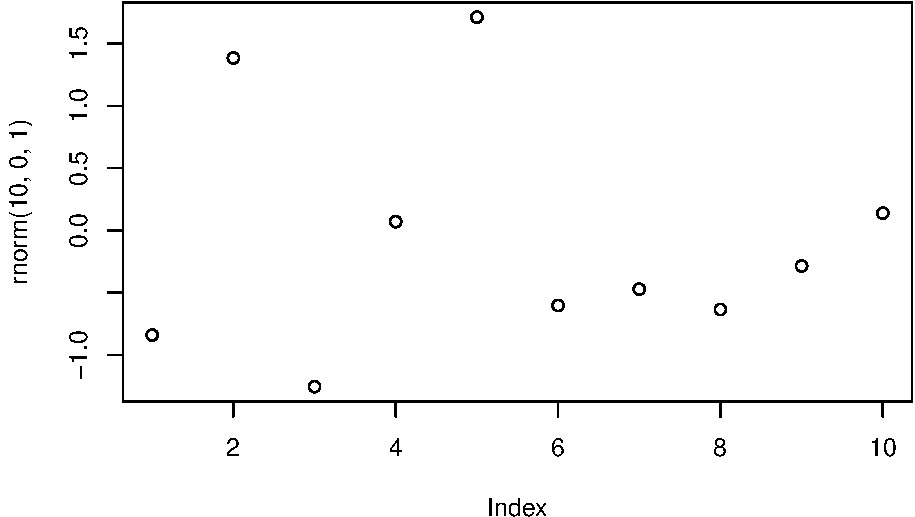
\includegraphics{figs/unnamed-chunk-9-1.pdf}
\caption{\label{fig:unnamed-chunk-9}this one will be a white noise process
and a random walk\label{noise}}
\end{figure}

\hypertarget{system-of-equations}{%
\subsection{System of Equations}\label{system-of-equations}}

Our discussion so far has focused on one variable. Before moving to two
or more variables we want to pause and highlight how much researchers
can explore with single variables. It is of course interesting and fun
to ask how two or more variables are related, or posit a complex
sequence among a set of variables. But understanding whether or not one
variable exhibits white noise or random walk behavior across time is a
valuable study in itself. We feel that our field could substantially
benefit from spending more time plotting and analyzing the individual
trajctories of every measured variable in a study.

With multivariate systems we need multiple equations -- one for each
variable. Before, we demonstrated a simple difference equation for
\(y\). In a multivariate system with two variables, \(x\) and \(y\), we
need one equation for each:

\begin{equation}
\label{sysy}
y_{t} = a y_{t - 1} + e_{t}
\end{equation} \begin{equation}
\label{sysx}
x_{t} = a x_{t - 1} + e_{t}
\end{equation}

\noindent where both equations posit that their variable is a function
of its prior self to the extent of the autoregressive term (\(a\)).
Notice that there are no cross-relationships, we are simply representing
a system with two independent variables across time. It is of course
also possible to introduce relationships among the different variables
with more terms.

First, consider a system where \(x\) concurrently causes \(y\). A more
appropriate way to say this would be that \(x_t\) causes \(y_t\):

\begin{equation}
\label{sysy2}
y_{t} = a y_{t - 1} + b x_{t} + e_{t}
\end{equation} \begin{equation}
\label{sysx2}
x_{t} = a x_{t - 1} + e_{t}
\end{equation}

\noindent where all terms are defined above but now the equation for
\(y\) also includes \(x_{t}\), the value of \(x\) and time \(t\), and
\(b\), the coefficient relating \(x\) to \(y\). This set of equations
says that \(x\) is simply a product of itself over time (with error),
whereas \(y\) is a function of itself and also \(x\) at the immediate
time point.

What if there is a lag between when \(x\) causes \(y\)? That is, perhaps
we posit that \(x\) does not immediately cause \(y\) but instead causes
\(y\) after some period of time. If the lag effect were 2, that would
mean that \(x_t\) causes \(y_{t + 2}\), and to express the \enquote{lag
2 effect} mathematically we would use the following.

\begin{equation}
\label{sysy3}
y_{t} = a y_{t - 1} + b x_{t - 2} + e_{t}
\end{equation} \begin{equation}
\label{sysx3}
x_{t} = a x_{t - 1} + e_{t}
\end{equation}

\noindent Here, all terms are nearly identical to what we saw above but
now there is a lag-two effect from \(x\) to \(y\). \(y\) is now a
function of both its immediately prior self and the value of \(x\) from
two time points ago.

What if we want to convey feedback, or a reciprocal relationship between
\(x\) and \(y\)? That is, now we posit that both \(x\) causes \(y\) and
\(y\) causes \(x\). To do so we update our equations with a simple
change:

\begin{equation}
\label{sysy3}
y_{t} = a y_{t - 1} + b x_{t - 2} + e_{t}
\end{equation} \begin{equation}
\label{sysx3}
x_{t} = a x_{t - 1} + b y_{t - 2} + e_{t}
\end{equation}

\noindent where all terms are defined above but now \(x\) and \(y\) are
reciprocally related. Both are determined by themselves at the
immediately prior time point and the other variable two time points in
the past. \(x\) happens, and two moments later this influences \(y\),
and two moments later this influences \(x\), and so on throughout time.
All the while, both variables retain self-similarity -- they change and
develop but only under the constraints afforded by the autoregressive
terms.

We can make the equations more complicated by continuing to add
variables or longer/shorter lag effects, but the beauty of math is its
freedom to capture whatever the researcher desires. These equations are
language tools to help researchers convey a process over time. If we
were to plug values into the coefficients and variables we would produce
trajectories over time, and to describe those trajectories we could then
use terms like \enquote{trend,} \enquote{periodicity,} or
\enquote{feedback} like we saw in the systems theory section.

\hypertarget{examples-1}{%
\subsection{Examples}\label{examples-1}}

People from our literature using these principles to explain something.
Study 1 argued for random walk behavior in X. Study 2 measured X and Y
and posited an equation.

\hypertarget{summary-1}{%
\subsection{Summary}\label{summary-1}}

\hypertarget{computational-principles}{%
\section{Computational Principles}\label{computational-principles}}

Above, we unpacked representations most people are familiar with: verbal
descriptions, plots, and math. There has recently been a push to use
computational models -- where the goal is still to convey process but in
computer code. In this section we discuss several principles that
researchers can use when they are explaining a process and expect that
explanation to eventually be evaluated with a computational model. We
are not going to show code or a set of scripts or \enquote{if
statements} (although doing so would be a valuable paper on its own).
Instead, the principles below are pieces that should be incoporated into
an explanation if the researcher hopes to eventually evaluate it in a
computer simulation. This section will also be different from the
sections above because we will use a running example throughout, and the
example comes from Simon (1956).

While developing his notion of satisficing Simon wrote a paper exploring
simple rules that could yield adaptive behavior. His paper was not
framed as a \enquote{computational model,} but his writing is a great
example of how authors can write verbal explanations that lend
themselves to computer simulations. Writing equations is of course
preferred, but the concepts below are tools/criteria for researchers
without a strong mathematical background.

\hypertarget{key-states}{%
\subsection{Key States}\label{key-states}}

Simon's (1956) paper is about how agents move through an environment and
choose among multiple goals -- it is about multiple goal
self-regulation. He begins by arguing that agents choose among multiple
goals to satisfy needs, and need satisfaction is the core driver of
behavior. There are of course other causes, but everything is done with
respect to the need requirements. The two needs he includes are food and
water.

Simon begins his explanation with needs, and although there are other
causes of behavior he makes the assumption that needs are the lowest
level of abstraction required to explain his model. They can be thought
of as the \enquote{foundation} variables to build from. Researchers
should be clear about the core variables that drive all other behavior
in their models. Variables are called \enquote{states} when we talk
about them over time, so the first principle is to adequately identify
and describe the key states.

\hypertarget{state-dynamics}{%
\subsection{State Dynamics}\label{state-dynamics}}

Once we identify the states we need to describe their behavior over
time. Again, Simon's (1956) key states are food and water, and he then
goes on to describe how they unfold as time progresses. He posits that
an agent's food and water states decrease over time because his or her
body requires energy. The body is constantly using food and water in its
stores, so as time passes the key states naturally decrease.

\hypertarget{actions}{%
\subsection{Actions}\label{actions}}

The key states are the assumed \enquote{proximate} causes of behavior,
and we have now explained how they unfold over time. Next, we need to
explain the list of possible behaviors that the causes lead to. In other
words, we need actions that result given the set of states and their
current dynamics. In Simon's model he lists three agent actions:
resting, exploring, and goal striving. These actions satisfy the
internal state dynamics. How so? That is the next criteria.

\hypertarget{action-selection}{%
\subsection{Action Selection}\label{action-selection}}

Assuming a set of actions, how does the agent select among them? Action
selection is the principle for explaining how one of the actions
actually occurs given the states and their dynamics. Simon argues that
if the food and water states are above threshold then the agent rests.
That is, he suggests that the food and water states act like stores
(although they constantly decrease) and only produce action when some
negative discrepancy exists. When one of the states dips below threshold
the agent explores its environment. During exploration the agent
randomly runs into objects, and if he or she encounters a single object
relevant to one of the needs the agent acquires it. If instead the agent
encounters two or more need-relevant objects he or she makes a decision
based on the ratio of effort required to get the object versus the size
of the state discrepancy. In summary, action selection is about how
behavior occurs given the states and their dynamics, whereas actions are
simply the names of the behaviors themselves.

\hypertarget{environment}{%
\subsection{Environment}\label{environment}}

Finally, computer simulations require a structure or environment for
agents to operate within. The environment could be a lattice, a
well-mixed population, or any number of network arrangements, but the
core idea is that context shapes what ultimately happens. Simon explains
his simple rules model within a grid that contains spatially distributed
sources of food and water. The size of the food and water stocks are
determined by the availability of the resources in the environment.
Water is easier to come by than food and so food requirements are
greater.

\hypertarget{summary-2}{%
\subsection{Summary}\label{summary-2}}

\hypertarget{discussion}{%
\section{Discussion}\label{discussion}}

Having presented the principles and terms like process, longitudinal,
and dynamics, we close with our opinion about how the term
\enquote{process} should be used. In our view, only explanations about
the proposed \enquote{true} mechanism should be called
\enquote{process.} If a researcher, instead, simply observes and
describes manifest behavior like trend or correlates of trend then they
are not explaining process -- but it is still a useful study!

\newpage

\hypertarget{references}{%
\section{References}\label{references}}

\setlength{\parindent}{-0.5in}
\setlength{\leftskip}{0.5in}

\hypertarget{refs}{}
\leavevmode\hypertarget{ref-aguinis_first_2009}{}%
Aguinis, H., Pierce, C. A., Bosco, F. A., \& Muslin, I. S. (2009). First
decade of Organizational Research Methods: Trends in design,
measurement, and data-analysis topics. \emph{Organizational Research
Methods}, \emph{12}(1), 69--112.

\leavevmode\hypertarget{ref-baltes_longitudinal_1979}{}%
Baltes, P. B., \& Nesselroade, J. R. (1979). \emph{Longitudinal research
in the study of behavior and development}. Academic Press New York, NY.

\leavevmode\hypertarget{ref-beal_esm_2015}{}%
Beal, D. J. (2015). ESM 2.0: State of the art and future potential of
experience sampling methods in organizational research. \emph{Annu. Rev.
Organ. Psychol. Organ. Behav.}, \emph{2}(1), 383--407.

\leavevmode\hypertarget{ref-cronin2009don}{}%
Cronin, M. A., Gonzalez, C., \& Sterman, J. D. (2009). Why don't
well-educated adults understand accumulation? A challenge to
researchers, educators, and citizens. \emph{Organizational Behavior and
Human Decision Processes}, \emph{108}(1), 116--130.

\leavevmode\hypertarget{ref-deshon_multivariate_2012}{}%
DeShon, R. P. (2012). Multivariate dynamics in organizational science.
\emph{The Oxford Handbook of Organizational Psychology}, \emph{1},
117--142.

\leavevmode\hypertarget{ref-hardy_interrelationships_2018}{}%
Hardy, J. H., Day, E. A., \& Steele, L. M. (2018). Interrelationships
Among Self-Regulated Learning Processes: Toward a Dynamic Process-Based
Model of Self-Regulated Learning. \emph{Journal of Management},
0149206318780440.
doi:\href{https://doi.org/10.1177/0149206318780440}{10.1177/0149206318780440}

\leavevmode\hypertarget{ref-ilgen_computational_2000}{}%
Ilgen, D. R., \& Hulin, C. L. (2000). \emph{Computational modeling of
behavior in organizations: The third scientific discipline.} American
Psychological Association.

\leavevmode\hypertarget{ref-johnson_good_2014}{}%
Johnson, R. E., Lanaj, K., \& Barnes, C. M. (2014). The good and bad of
being fair: Effects of procedural and interpersonal justice behaviors on
regulatory resources. \emph{Journal of Applied Psychology},
\emph{99}(4), 635.

\leavevmode\hypertarget{ref-mcelreath_statistical_2016}{}%
McElreath, R. (2016). \emph{Statistical Rethinking: A Bayesian Course
with Examples in R and Stan} (Vol. 122). CRC Press.

\leavevmode\hypertarget{ref-meadows2008thinking}{}%
Meadows, D. H. (2008). \emph{Thinking in systems: A primer}. chelsea
green publishing.

\leavevmode\hypertarget{ref-monge_theoretical_1990}{}%
Monge, P. R. (1990). Theoretical and analytical issues in studying
organizational processes. \emph{Organization Science}, \emph{1}(4),
406--430.

\leavevmode\hypertarget{ref-pettigrew_character_1992}{}%
Pettigrew, A. M. (1992). The character and significance of strategy
process research. \emph{Strategic Management Journal}, \emph{13}(S2),
5--16.

\leavevmode\hypertarget{ref-pettigrew_what_1997-1}{}%
Pettigrew, A. M. (1997). What is a processual analysis?
\emph{Scandinavian Journal of Management}, \emph{13}(4), 337--348.
doi:\href{https://doi.org/10.1016/S0956-5221(97)00020-1}{10.1016/S0956-5221(97)00020-1}

\leavevmode\hypertarget{ref-ployhart_longitudinal_2010}{}%
Ployhart, R. E., \& Vandenberg, R. J. (2010). Longitudinal research: The
theory, design, and analysis of change. \emph{Journal of Management},
\emph{36}(1), 94--120.

\leavevmode\hypertarget{ref-schaubroeck_can_2016}{}%
Schaubroeck, J. M., Lam, S. S., \& Peng, A. C. (2016). Can peers'
ethical and transformational leadership improve coworkers' service
quality? A latent growth analysis. \emph{Organizational Behavior and
Human Decision Processes}, \emph{133}, 45--58.

\leavevmode\hypertarget{ref-shipp_time_2015}{}%
Shipp, A. J., \& Cole, M. S. (2015). Time in individual-level
organizational studies: What is it, how is it used, and why isn't it
exploited more often? \emph{Annu. Rev. Organ. Psychol. Organ. Behav.},
\emph{2}(1), 237--260.

\leavevmode\hypertarget{ref-simon1956rational}{}%
Simon, H. A. (1956). Rational choice and the structure of the
environment. \emph{Psychological Review}, \emph{63}(2), 129.

\leavevmode\hypertarget{ref-vancouver_translating_2018}{}%
Vancouver, J. B., Wang, M., \& Li, X. (2018). Translating Informal
Theories Into Formal Theories: The Case of the Dynamic Computational
Model of the Integrated Model of Work Motivation. \emph{Organizational
Research Methods}, 109442811878030.
doi:\href{https://doi.org/10.1177/1094428118780308}{10.1177/1094428118780308}

\leavevmode\hypertarget{ref-Wang2016}{}%
Wang, M., Zhou, L., \& Zhang, Z. (2016). Dynamic modeling. \emph{Annual
Review of Organizational Psychology and Organizational Behavior},
\emph{3}(1), 241--266.
doi:\href{https://doi.org/10.1146/annurev-orgpsych-041015-062553}{10.1146/annurev-orgpsych-041015-062553}


\end{document}
